
\section{Preliminaries}
I begin by providing definitions needed to understand the inverse problem presented by Grindrod et al. in ~\cite{grindrod2009}.
In particular, they wish to fit a series of states of the graph $G$ by fitting them to a model.
One model for this is a model of birth rates and death rates.
For each pair of vertices $u,v \in G$, I want to assign the following:
\begin{itemize}
	\item Birth Rate $\alpha (u, v)$: The probability of the edge $u-v$ appearing if it does not exist in the current state.
	\item Death Rate $\omega (u,v)$: The probability of the edge $u-v$ disappearing if it exists in the current state.
\end{itemize}

To find a reasonable assignment for these birth and death rates, I use the idea of range-dependent graphs.

\begin{definition} \label{def:range}
	Range-dependent graphs are an assignment of the integers $q = \{1,2,\dots,n\}$ on $n$ vertices such that, for each vertex, the range
	between two vertices is defined as $|q(u) - q(v)|$.
\end{definition}

I can use this definition of range as a way to determine the probability of two vertices having an edge. 
The smaller the range between two vertices, the more likely that they should have an edge.

\begin{figure}
	\begin{center}
		\begin{tikzpicture}
    \tikzstyle{node} = [circle, fill=lightgray!90!black, draw, thick]
    \tikzstyle{edge} = [thick]
    \tikzstyle{edit} = [fill=editcol]
    \tikzstyle{lift} = [fill=liftcol]

    \node (1) [node] {1};
    \node (2) [node, right=0.3cm of 1] {2};
    \node (3) [node, right=0.3cm of 2] {3};
    \node (4) [node, right=0.3cm of 3] {4};

    \draw (1) edge [edge] (2);
    \draw (2) edge [edge] (3);
    \draw (3) edge [edge] (4);

\end{tikzpicture}
	\end{center}
	\caption{
		A path showcasing an assignment of ranges on the vertices.
		Vertex 1 and vertex 4 have a range of $4-1 = 3$, whereas
		vertex 1 and vertex 2 have a range of $2-1=1$.
	}
	\label{fig:range}
\end{figure}

\begin{figure}
	\begin{center}
		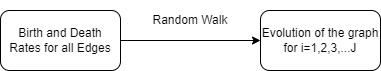
\includegraphics{figures/Inverse Problem Figure.jpg}
	\end{center}
	\caption{
		This figure defines the inverse problem I am aiming to solve.
	}
	\label{fig:inverse}
\end{figure}

This brings us to the inverse problem I wish to solve.
Given $J$ states of the graph $G$, we wish to learn a range assignment $q$ on the vertices such that the error is minimized.
Refer to Figure ~\ref{fig:inverse} for a depiction of the inverse problem.

Formally, the problem is defined as follows:

\begin{problem}{Evolving Graph Model}
	\Input & $J$ states of the graph $G$ and a matrix $R$ containing the frequencies of each edge in $G$\\
	\Prob & What mapping on the integers $q$ minimizes $\sum_{v_1,v_2 \in G}R[v_1][v_2](q(v_1) - q(v_2))^2$?
\end{problem}

By solving this problem, I can use the range mapping $q$ to define birth and death rates that make reasonable predictions for
future evolutions of $G$.
As $q$ is a non-differentiable function as a mapping, a solution here is not well defined.
The problem can be relaxed by considering $q$ as a vector.
This creates the quadratic inverse problem of $q^T \Delta_R q$.
Grindrod et al. ~\cite{grindrod2009} solve this problem via complex eigenanalysis.
The rest of this report concerns my results in applying methods from the course on this inverse problem.